
\subsection{Liczba warkoczowa}
\index{liczba warkoczowa|(}%

% DICTIONARY;braid number;liczba warkoczowa;-
\begin{definition}
\label{def:braid_number}%
    Niech $L$ będzie splotem.
    Najmniejszą liczbę pasm, na których można zapleść warkocz $b$, którego domknięciem jest splot $L$, nazywamy liczbą warkoczową splotu $L$.
\end{definition}

Tylko jeden węzeł ma liczbę warkoczową $1$, jest to niewęzeł.
Dwuwarkoczowe są dokładnie węzły torusowe typu $(2, n)$ dla $|n| \ge 3$.
Węzły spełniające $\braid (K) = 3$ nie zostały jeszcze sklasyfikowane.
Liczba warkoczowa splotu zależy od orientacji ogniw (patrz rysunek poniżej) i~trudno wyznacza się w~ogólnym przypadku.
Znamy ją między innymi dla węzłów torusowych (fakt~\ref{cor:torus_braid_number}).

\begin{comment}
    \begin{figure}[H]
        \centering
        \begin{minipage}[b]{.24\linewidth}
            \centering
            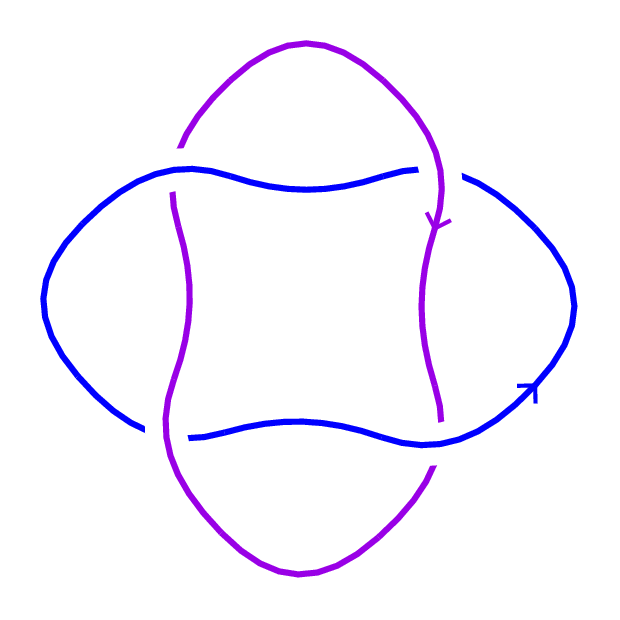
\includegraphics[width=\linewidth]{../data/links/l4a1-0.png}
            \subcaption{$\braid (L_4a_{1, 0}) = 3$}
        \end{minipage}
        \begin{minipage}[b]{.24\linewidth}
            \centering
            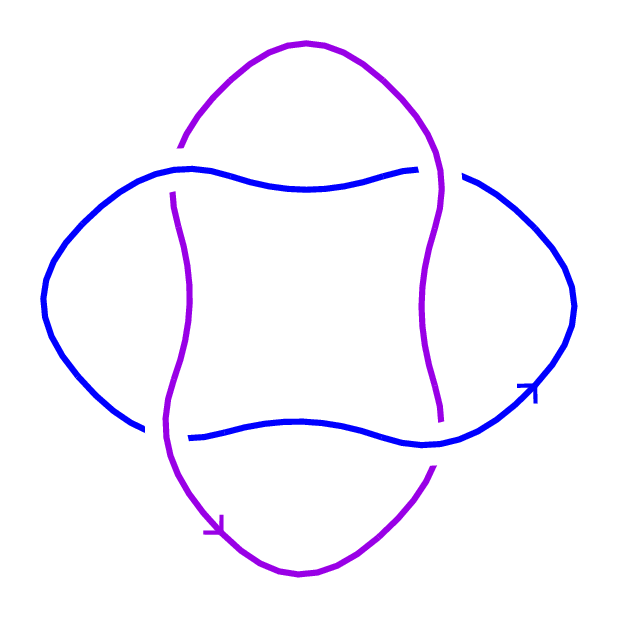
\includegraphics[width=\linewidth]{../data/links/l4a1-1.png}
            \subcaption{$\braid (L_4a_{1, 1}) = 2$}
        \end{minipage}
        \begin{minipage}[b]{.24\linewidth}
            \centering
            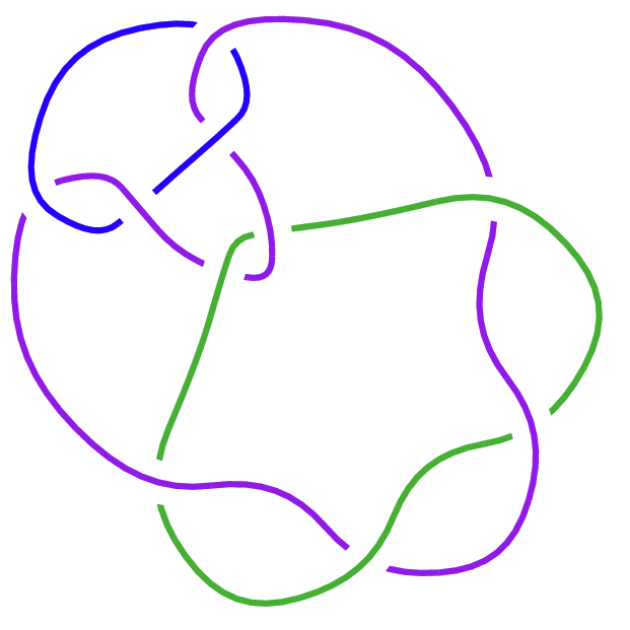
\includegraphics[width=\linewidth]{../data/links/l10a153-u.png}
            \subcaption{$L_{10}a_{153}$}
        \end{minipage}
        \caption{Liczba warkoczowa splotu zależy od orientacji}
    \end{figure}
\end{comment}

Według bazy danych LinkInfo\footnote{\url{https://linkinfo.sitehost.iu.edu/index.php} (sprawdzono 8 listopada 2023 roku).} istnieją 1424 niezorientowane sploty pierwsze o indeksie skrzyżowaniowym 11 lub mniejszym.
% TODO: zamienić na prawdziwe cytowanie
Spośród nich, 622 sploty mają tę samą liczbę warkoczową niezależnie od tego, jak zorientowane są ich ogniwa.   
Z drugiej strony dokładnie jeden splot z~bazy LinkInfo, $L_{10}a_{153}$, może mieć aż cztery różne liczby warkoczowe: 3, 4, 5 lub 6.

\begin{proposition}
    Węzeł o~$n$ skrzyżowaniach można zapleść na $n - 1$ pasmach: $\crossing K \ge 1 + \braid K$.
\end{proposition}

Powyższe ograniczenie nie jest zbyt użyteczne, równość mamy jedynie dla trójlistnika i~ósemki.
Ohyama \cite{ohyama1993} pokazał:
\index[persons]{Ohyama, Yoshiyuki}%

\begin{proposition}
    Niech $L$ będzie nierozszczepialnym splotem.
    Wtedy $\crossing L \ge 2 \braid L - 2$.
\end{proposition}

Dowód korzysta z grafu Seiferta splotu.
\index{graf Seiferta}%
Wśród pierwszych węzłów do 10 skrzyżowań mamy równość dziesięć razy: dla $4_1$, $6_1$, $8_1$, $8_3$, $8_{12}$, $10_1$, $10_3$, $10_{13}$, $10_{35}$, $10_{58}$.
%=% PANDAS
%=% >>> knots = [x for x in d.query('crossing_number == 2 * braid_index - 2 and crossing_number < 11')["name"]]; print(len(knots), knots)
%=% 10 ['4_1', '6_1', '8_1', '8_3', '8_12', '10_1', '10_3', '10_13', '10_35', '10_58']
% TODO: czemu tutaj?

\begin{proposition}[nierówność Mortona-Franksa-Williamsa]
\index{nierówność Mortona-Franksa-Williamsa}%
    Niech $L$ będzie zorientowanym splotem, zaś $\operatorname{span}_\alpha$ różnicą między największym i najmniejszym stopniem zmiennej $\alpha$ wielomianu HOMFLY zmiennych $\alpha, z$.
    Wtedy
    \begin{equation}
        \braid L \ge 1 + \frac 1 2 \operatorname{span}_\alpha P(\alpha, z).
    \end{equation}
\end{proposition}

Nierówność jest ostra dla wszystkich pierwszych węzłów do 10 skrzyżowań poza $9_{42}$, $9_{49}$, $10_{132}$, $10_{150}$ oraz $10_{156}$.
Dowód podali niezależnie Franks, Williams \cite{franks1987} i Morton \cite{morton1988}.
\index[persons]{Franks, John}%
\index[persons]{Morton, Hugh}%
\index[persons]{Williams, Robert}%
% TODO: zweryfikować z ./tools/knotinfo_parsed.json programem w Pythonie

Wielomian Alexandera wykrywa czasami węzły, których nie otrzyma się przez domykanie ,,małych'' warkoczy.
\index{wielomian!Alexandera}%
Przytoczone tu wyniki pochodzą z pracy Jonesa \cite{jones1985}, gdzie nie ma jednak ich dowodów.

\begin{proposition}
    Jeśli $|\alexander_K(i)| > 3$, to węzeł $K$ nie jest domknięciem 3-warkocza.
\end{proposition}

Ta implikacja, \cite[wniosek 23]{jones1985}, jest skuteczna przy 43 z 59 węzłów pierwszych o mniej niż 10 skrzyżowaniach.
Jones \cite[wniosek 24]{jones1985} zasugerował, że domknięcia 4-warkoczy spełniają podobną nierówność $|\alexander (\exp (2\pi i / 5))| \le 13/2$, ale Stojmenow \cite{stoimenow2002} odkrył po wielu latach, dlaczego nikt nigdy nie podał dowodu tego faktu.
Węzeł $13_{9221}$ ma liczbę warkoczową 4, jego wielomian Alexandera przyjmuje wartość $\alexander(\omega_5) = 19\sqrt{5} - 49 \approx -6.51$.

Udało mu się za to udowodnić słabszą implikację ($6 + 2 \sqrt{5} \approx 10.47$):

\begin{proposition}
    Jeśli $|\alexander_K(\exp(2\pi i/5))| > 6 + 2 \sqrt{5}$, to węzeł $K$ nie jest domknięciem 4-warkocza.
\end{proposition}

Prawdopodobnie nie istnieją podobne warunki dla 5-warkoczy.

\index{liczba warkoczowa|)}%

% Koniec podsekcji Liczba warkoczowa

